\documentclass[../main.tex]{subfiles}
\begin{document}
\chapter{Basics Of Vectors}
\section{Definition and Axioms}
\subsection{Introductory Definitions}
A vector is specified by a (positive) magnitude and a direction in space.
We can represent a vector as line segment between two points $A$ and $B$, $\vec{v} = \avec{AB}$.
$\vec{v}$ has length $|\vec{v}|$ and direction from $A$ to $B$.
If we chose an origin $O$ then considering a point $A$ it has position vector denoted $\vec{a} = \avec{OA}$.
\begin{definition}[Vector Space]
  A \textit{vector space}, $V$, over $\R$ or $\C$ is a collection of vectors $\vec{v} \in V$, together with two operations:
  \begin{enumerate}
    \item Addition of two vectors
    \item Multiplication by a scalar (from $\R$ or $\C$ respectively)
  \end{enumerate}
\end{definition}
Vector addition has to satisfy the following axioms:
\begin{enumerate}
  \item \textbf{Commutativity -} $\vec{a} + \vec{b} = \vec{b} + \vec{a}$
  \item \textbf{Associativity -} $(\vec{a} + \vec{b}) + \vec{c} = \vec{a} + (\vec{b} + \vec{c})$
  \item \textbf{Identity -} There exists a vector $\vec{0}$ such that for all $a \in V$, $\vec{a} + \vec{0} = \vec{a}$
  \item \textbf{Inverse -} For all vectors $\vec{a} \in V$, there is a vector ($-\vec{a}$) such that $\vec{a} + (-\vec{a}) = \vec{0}$.
\end{enumerate}
Scalar multiplication has to satisfy the following axioms (Where $\lambda$ and $\mu$ are scalars):
\begin{enumerate}
  \item $\lambda(\vec{a} + \vec{b}) = \lambda \vec{a} + \lambda \vec{b}$
  \item $(\lambda + \mu)\vec{a} = \lambda \vec{a} + \mu \vec{a}$
  \item $\lambda(\mu \vec{a}) = (\lambda \mu)\vec{a}$
  \item $1(\vec{a}) = \vec{a}$
\end{enumerate}
\begin{remark}
  Vectors under addition are an abelian group.
\end{remark}
\begin{remark}[Warning]
  $\R^{n}$ is a vector space with addition (component-wise) and scalar multiplication.
  We can represent $\R$ by a line and this could make us think that any line is a vector space however this is not true as the space does not necessarily contain $O$.
  E.g. $x + y = d$ is not a vector space.
\end{remark}

\subsection{Geometric View}
Given vectors $\vec{a}$ and $\vec{b}$ which are the position vectors of $A$ and $B$ respectively, we can construct the parallelogram $OACB$:
\begin{center}
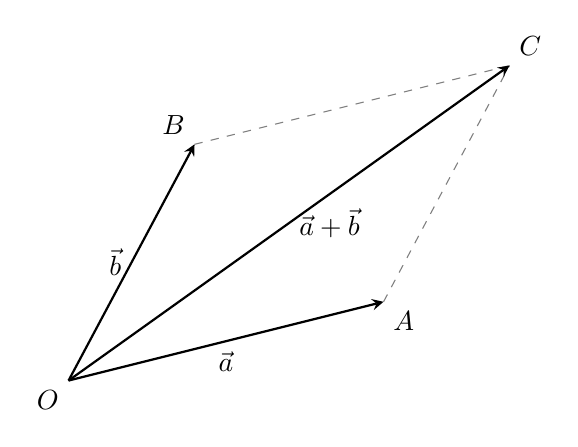
\begin{tikzpicture}[scale=2,>=stealth]
  \coordinate (O) at (0,0);
  \coordinate (A) at (2,0.5);   % vector a
  \coordinate (B) at (0.8,1.5); % vector b
  \coordinate (C) at (2.8,2);   % a + b

  \node[below left] at (O) {$O$};
  \node[below right] at (A) {$A$};
  \node[above left] at (B) {$B$};
  \node[above right] at (C) {$C$};

  \draw[->, thick, black] (O) -- (A) node[midway, below] {$\vec{a}$};
  \draw[->, thick, black] (O) -- (B) node[midway, left] {$\vec{b}$};

  \draw[dashed, gray] (A) -- (C);
  \draw[dashed, gray] (B) -- (C);

  \draw[->, thick, black] (O) -- (C) node[midway, right] {$\vec{a} + \vec{b}$};
\end{tikzpicture}
\end{center}

and then $\vec{a} + \vec{b} = \vec{c}$, where $\vec{c}$ is the position vector of $C$.

Given a vector $\vec{a}$ which is the position vector of a point $A$ and a $\lambda \in \R$.
$\lambda \vec{a}$ is a position vector of a point on the line through $OA$, with length $|\lambda \vec{a}| = |\lambda||\vec{a}$.

\begin{center}
\begin{tikzpicture}[scale=2,>=stealth]
  \coordinate (O) at (0,0);
  \coordinate (A) at (1.2,0.6);
  \coordinate (B) at (2.4,1.2);
  \coordinate (C) at (-1.2,-0.6);

  % Guide line
  \draw[dashed, gray] (-1.6,-0.8) -- (3,1.5);

  % Original vector
  \draw[->, thick, black] (O) -- (A) node[midway, below right] {$\vec{a}$};

  % Scaled vector
  \draw[->, black] (O) -- (B) node[near end, below right] {$\lambda \vec{a}$};

  % Reversed vector
  \draw[->, black] (O) -- (C) node[near end, below right] {$-\frac{\lambda}{2} \vec{a}$};

  % Label points
  \fill (O) circle (0.03);
  \node[below right] at (O) {$O$};
  \node[below right] at (A) {$A$};
\end{tikzpicture}
\end{center}
\begin{remark}[Note]
  $\{\lambda \vec{a}: \lambda \in \R\}$ is the set of all points on the line through $OA$.
\end{remark}

\subsection{Linear Combination and Span}
\begin{definition}[Linear Combination]
  Given $n$ vectors $\vec{r}_1, \vec{r}_2, \ldots, \vec{r}_n$, a \textit{linear combination} of those vectors is a vector of the form:
  \[
    \sum_{i = 1}^{n} \lambda_i \vec{r}_i  = \lambda_1 \vec{r}_1 + \lambda_2 \vec{r}_2 + \cdots + \lambda_n \vec{r}_n
  \]
  where $\lambda_1, \lambda_2, \ldots, \lambda_n$ are scalars.
\end{definition}
We can also define the ``space'' of all linear combinations of a set of vectors:
\begin{definition}[Span]
  Given $n$ vectors $\vec{r}_1, \vec{r}_2, \ldots, \vec{r}_n$, their \textit{span} is the set of all linear combinations of those vectors.
  \[
    \Span\{\vec{r}_1, \vec{r}_2, \ldots, \vec{r}_n\} = \left\{\sum_{i = 1}^{n} \lambda_i \vec{r}_i : \lambda_i \in K\right\}
  \]
  where $K$ is either $\C$ or $\R$ depending on the vector space.
\end{definition}
\begin{definition}[Parallel]
  Any two vectors $\vec{a}$ and $\vec{b}$ are \textit{parallel} if $\vec{a} = \lambda \vec{b}$ or $\vec{b} = \lambda \vec{a}$ for some $\lambda \in \R$.
  We denote this $\vec{a} \parallel \vec{b}$.
\end{definition}
\begin{remark}[Note]
  Since we allow $\lambda = 0$, $\vec{0} \parallel \vec{a}$ for any $\vec{a}$.
\end{remark}
If $\vec{a} \centernot\parallel \vec{b}$ ($\vec{a}$ and $\vec{b}$ are not parallel), then $\Span\{\vec{a}, \vec{b}\}$ is a plane through $O$, $A$, and $B$.
\begin{definition}[Unit Vector]
  A \textit{unit vector} is a vector with length $1$.
  They are denoted $\uvec{v}$.
\end{definition}
\section{Scalar Product}
The \textit{scalar product} of two vectors within a vector space returns a scalar (either real or complex).
\subsection{Geometric Viewpoint in \texorpdfstring{$\R^{n}$}{Real Vector Spaces}}
First consider the usual scalar product in $\R^{n}$.
\begin{definition}[Scalar Product]
  The \textit{scalar product} of two vectors $\vec{a}$ and $\vec{b}$ is defined as:
  \[
    \vec{a} \cdot \vec{b} = |\vec{a}||\vec{b}|\cos\theta
  \]
  where $\theta$ is the angle between $\vec{a}$ and $\vec{b}$.
\end{definition}
\begin{remark}[Note]
  If $|\vec{a}| = 0$ or $|\vec{b}| = 0$ then $\theta$ is not well defined, but in that case we have $\vec{a} \cdot \vec{b} = 0$.
\end{remark}
Intuitively the dot product is the product of the parts of $\vec{a}$ and $\vec{b}$ that are parallel.

The scalar product in $\R^{n}$ satisfies the following properties:
\begin{enumerate}
  \item $\vec{a} \cdot \vec{b} = \vec{b} \cdot \vec{a}$
  \item $\vec{a} \cdot \vec{a} = |\vec{a}|^2 \geq 0$ (and $|\vec{a}| = 0 \iff \vec{a} = \vec{0}$)
  \item $(\lambda \vec{a}) \cdot \vec{b} = \lambda (\vec{a} \cdot \vec{b}) = \vec{a} \cdot (\lambda \vec{b})$
  \item $\vec{a} \cdot (\vec{b} + \vec{c}) = \vec{a} \cdot \vec{b} + \vec{a} \cdot \vec{c}$
\end{enumerate}
\begin{definition}[Orthogonal]
  Any two vectors $\vec{a}$ and $\vec{b}$ are \textit{orthogonal} or \textit{perpendicular} if $\vec{a} \cdot \vec{b} = 0$.
  We denote this $\vec{a} \perp \vec{b}$.
\end{definition}
\begin{remark}[Note]
  We also also allow $\vec{a} = \vec{0}$ or $\vec{b} = \vec{0}$ and hence $\vec{0}$ is orthogonal to any other vector.
\end{remark}
\begin{definition}[Projection]
  Given two vectors $\vec{a}$ and $\vec{b}$, the projection of $\vec{b}$ onto $\vec{a}$ is:
  \[
    \uvec{a}|\vec{b}|\cos \theta = (\uvec{a} \cdot \vec{b}) \uvec{a}
  \]
\end{definition}

\begin{center}
\begin{tikzpicture}[scale=2,>=stealth]
  \coordinate (O) at (0,0);
  \coordinate (A) at (2,0);
  \coordinate (B) at (1.2,1.4);
  \coordinate (P) at (1.2,0);

  % vectors a and b
  \draw[->, black] (O) -- (A) node[near end, below] {$\vec{a}$};
  \draw[->, black] (O) -- (B) node[midway, left] {$\vec{b}$};

  % projection line
  \draw[dashed, gray] (B) -- (P);

  % projection of b onto a
  \draw[->, thick, black] (O) -- (P) node[midway, below] {$\underbrace{(|\vec{b}|\cos\theta)\uvec{a}}_{\text{projection of $\vec{b}$ onto $\vec{a}$}}$};

  % angles
  \draw (0.5,0) arc[start angle=0, end angle=49, radius=0.5];
  \node at (0.6,0.2) {$\theta$};
  \draw ($(P)+(0,0.1)$) -- ($(P)+(0.1,0.1)$) -- ($(P)+(0.1,0)$);
\end{tikzpicture}
\end{center}
We can use the scalar product to quickly derive the cosine rule:
\begin{proof}
  \begin{align*}
    |\avec{BC}|^2 &= |\avec{AC} - \avec{AB}|^2 \\
                  &= (\avec{AC} - \avec{AB}) \cdot (\avec{AC} - \avec{AB}) \\
                  &= |\avec{AC}|^2 - 2 \avec{AB} \cdot \avec{AC} + |\avec{AB}|^2 \\
                  &= |\avec{AC}|^2 + |\avec{AB}|^2 - 2 |\avec{AB}||\avec{AC}|\cos\theta
  \end{align*}
\end{proof}
\subsection{General Algebraic Viewpoint}
This definition generalises to any other vector space, keeping the same axioms.
\begin{definition}[Inner/Scalar Product]
  In a real vector space $V$, an \textit{inner product} or \textit{scalar product} is a map $V \times V \to \R$ that satisfies:
  \begin{enumerate}
    \item \textbf{Symmetry -} $\vec{x} \cdot \vec{y} = \vec{y} \cdot \vec{x}$
    \item \textbf{Linearity in 2nd Argument -} $\vec{x} \cdot(\lambda \vec{y} + \mu \vec{z}) = \lambda \vec{x} \cdot \vec{y} + \mu \vec{x} \cdot \vec{z}$
    \item \textbf{Positive Definiteness - } $\vec{x} \cdot \vec{x} \geq 0$ with equality if and only if $\vec{x} = \vec{0}$
  \end{enumerate}
  We denote it either $\vec{x} \cdot \vec{y}$ or $\inner{\vec{x}}{\vec{y}}$.
\end{definition}
\begin{remark}[Note]
  We get linearity in the first argument also because of symmetry.
\end{remark}
\begin{definition}[Norm]
  The norm of a vector $\vec{a}$ is given by $\sqrt{\vec{a} \cdot \vec{a}}$.
  We denote this as either $|\vec{a}|$ or $\norm{\vec{a}}$.
\end{definition}
\begin{theorem}[Cauchy-Schwarz Inequality]
  For all $\vec{x}, \vec{y} \in \R^{n}$,
  \[
    |\vec{x} \cdot \vec{y}| \leq |\vec{x}||\vec{y}|
  \]
\end{theorem}
\begin{proof}
  Consider the expression $|x - \lambda y|^2$, $\lambda \in \R$.
  Then,
  \begin{align*}
    |\vec{x} - \lambda\vec{y}|^2 &\geq 0 \\
    (\vec{x} - \lambda \vec{y}) \cdot (\vec{x} - \lambda \vec{y}) &\geq 0 \\
    \abs{\vec{x}}^2 + \lambda^2 \abs{\vec{y}}^2 - 2\lambda \vec{x} \cdot \vec{y} &\geq 0 \\
    (\lambda^2 \abs{\vec{y}}^2 - 2 \vec{x} \cdot \vec{y} \lambda + \abs{\vec{x}}^2) &\geq 0
  \end{align*}
  This quadratic always needs to be non-negative so we require the discriminant to be less than or equal to zero.
  \begin{align*}
    4(\vec{x} \cdot \vec{y})^2 - 4 \abs{\vec{x}}^2 \abs{\vec{y}}^2 &\leq 0 \\
    \abs{\vec{x} \cdot \vec{y}} &\leq \abs{\vec{x}} \abs{\vec{y}}
  \end{align*}
\end{proof}
Notice that this proof holds for all possible scalar products on any real vector space as we only used the axioms of the scalar product.
\begin{remark}
  Equality ($\abs{\vec{x} \cdot \vec{y}} = \abs{\vec{x}}\abs{\vec{y}}$) holds if and only if $\vec{x} = \lambda \vec{y}$ or $\vec{y} = \lambda \vec{x}$ for some $\lambda \in \R$ (i.e. $\vec{x}$ and $\vec{y}$ are parallel).
\end{remark}
We can now set:
\[
  \vec{x} \cdot \vec{y} = |\vec{x}||\vec{y}|\cos\theta
\]
to define the angle between $\vec{x}$ and $\vec{y}$ in $\R^{n}$ since Cauchy-Schwarz ensures that $-1 \leq \cos \theta \leq 1$.
\begin{corollary}[Triangle Inequality]
  For two vectors $\vec{x}, \vec{y}$
  \[
    \abs{\vec{x} + \vec{y}} \leq \abs{\vec{x}} + \abs{\vec{y}}
  \]
\end{corollary}
\begin{proof}
  \begin{align*}
    \abs{\vec{x} + \vec{y}}^2 &= (\vec{x} + \vec{y}) \cdot (\vec{x} + \vec{y}) \\
                              &= \abs{\vec{x}}^2 + \abs{\vec{y}}^2 + 2 \vec{x} \cdot \vec{y} \\
                              &\leq \abs{\vec{x}}^2 + \abs{\vec{y}}^2 + 2 \abs{\vec{x}}\abs{\vec{y}} \\
                              &= (\abs{\vec{x}} + \abs{\vec{y}})^2
  \end{align*}
  Therefore $\abs{\vec{x} + \vec{y}} \leq \abs{\vec{x}} + \abs{\vec{y}}$.
\end{proof}

\section{Orthonormal Bases}
\begin{remark}[Note]
For this section, consider vectors in $\R^{3}$ only.
\end{remark}
Consider vectors $\vec{e}_1, \vec{e}_2, \vec{e}_3$ that are orthonormal:
\[
  \abs{\vec{e}_1} = \abs{\vec{e}_2} = \abs{\vec{e}_3} = 1 \text{ and } \vec{e}_i \cdot \vec{e}_j = \begin{cases}
  1 & i=j \\
  0 & i\neq j
  \end{cases}
\]
That is, they are all length 1 and are mutually orthogonal.
This is called an \textit{orthonormal basis} and is equivalent to choosing Cartesian axes along these directions.
There are infinitely many choices for an orthonormal basis in $\R^{3}$.

Any vector in $\R^{3}$ can be written as a combination of these:
\[
  \vec{a} = \sum_{i}^{} a_i \vec{e}_i = a_1 \vec{e}_1 + a_2 \vec{e}_2 + a_3 \vec{e}_3
\]
Each component of $\vec{a}$ is uniquely determined by $a_i = \vec{e}_i \cdot \vec{a}$

We will denote $\vec{a}$ as either a row vector or a column vector:
\[
  \vec{a} = (a_1, a_2, a_3) \text{ or } \vec{a} =
  \begin{pmatrix}
  a_1 \\
  a_2 \\
  a_3 \\
  \end{pmatrix}
\]
Now for $\vec{a}, \vec{b} \in \R^{3}$:
\begin{align*}
  \vec{a} \cdot \vec{b} &= (a_1 \vec{e}_1 + a_2 \vec{e}_2 + a_3 \vec{e}_3) \cdot (b_1 \vec{e}_1 + b_2 \vec{e}_2 + b_3 \vec{e}_3) \\
                        &= a_1 b_1 + a_2 b_2 + a_3 b_3
\end{align*}
In particular:
\[
  \vec{a} \cdot \vec{a} = \abs{\vec{a}}^2 = a^{2}_{1} + a^{2}_{2} + a^{2}_{3}
\]

The \textit{canonical basis} of $\R^{3}$, the one we use for the representation in terms of row or column vectors is:
\[
  \vec{e}_1 = (1, 0, 0),\; \vec{e}_2 = (0, 1, 0),\; \vec{e}_3 = (0, 0, 1)
\]
\begin{remark}[Notation]
The canonical orthonormal basis vectors for $\R^{3}$ are usually denoted $\uvec{i}$, $\uvec{j}$, $\uvec{k}$.
\end{remark}

\section{Vector Product}
\begin{remark}[Note]
For this section, consider vectors in $\R^{3}$ only.
\end{remark}
\subsection{Definition}
\begin{definition}[Vector Product]
  Consider $\vec{a}, \vec{b} \in \R^{3}$. The \textit{vector product} is defined by:
  \[
    \vec{a} \times \vec{b} = \abs{\vec{a}} \abs{\vec{b}}(\sin\theta)\uvec{n}
  \]
  Where $\uvec{n}$ is a unit vector that is orthogonal to both $\vec{a}$ and $\vec{b}$ and $\theta$ is the angle between $\vec{a}$ and $\vec{b}$.
  It is sometimes denoted $\vec{a} \wedge \vec{b}$.
\end{definition}
\begin{remark}[Right-Hand Rule]
  If $\vec{a}$ is on your first finger and $\vec{b}$ is on your second finger then $\vec{a} \times \vec{b}$ points in the direction of your thumb.
\end{remark}

\begin{center}
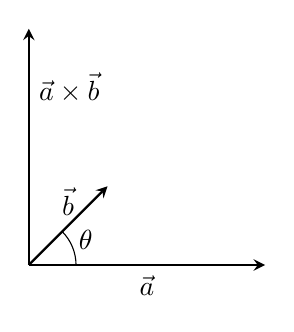
\begin{tikzpicture}[>=stealth]
\draw[thick,->] (0,0) -- (3,0) node[midway,below] {$\vec{a}$};
\draw[thick,->] (0,0) -- (1,1) node[midway,above] {$\vec{b}$};
\draw[thick,->] (0,0) -- (0,3) node[near end,right] {$\vec{a}\times \vec{b}$};
\draw (0.6,0) arc [start angle=0,end angle=45,radius=0.6] node[pos=0.7,right] {$\theta$};
\end{tikzpicture}
\end{center}
\begin{remark}
  $\uvec{n}$ is not defined if $\vec{a}$ and $\vec{b}$ are parallel but $\theta = 0 \text{ or } \pi$ so $\vec{a} \times \vec{b} = \vec{0}$.

  $\theta$ is not defined if $\abs{\vec{a}} = 0$ or $\abs{\vec{b}} = 0$ but then $\vec{a} \times \vec{b} = \vec{0}$ regardless.
\end{remark}
Some properties of the vector product are:
\begin{enumerate}
  \item $\vec{a} \times \vec{b} = - \vec{b} \times \vec{a}$ (Anti-symmetric)
  \item $\vec{a} \times \vec{a} = \vec{0}$
  \item $\vec{a} \times \vec{b} = 0 \iff \vec{a} = \lambda \vec{b}$ for some $\lambda \in \R$
  \item $(\lambda \vec{a}) \times \vec{b} = \lambda (\vec{a} \times \vec{b}) = \vec{a} \times (\lambda \vec{b})$
  \item $\vec{a} \times (\vec{b} + \vec{c}) = \vec{a} \times \vec{b} + \vec{a} \times \vec{c}$
  \item $\vec{a} \cdot (\vec{a} \times \vec{b}) = \vec{b} \cdot (\vec{a} \times \vec{b}) = 0$
\end{enumerate}
\subsection{Geometric Uses}
For vectors $\vec{a}, \vec{b}$ then $\vec{a} \times \vec{b}$ is the vector area of the parallelogram.
For example with $\sin \theta \geq 0$ we have:
\[
  \abs{\vec{a} \times \vec{b}} = \abs{\vec{a}} \abs{\vec{b}} \sin \theta = \text{base} \times \text{perpendicular height} = \text{area}
\]
\begin{center}
\begin{tikzpicture}[scale=3,>=stealth]
\coordinate (O) at (0,0);
\coordinate (A) at (2,0);
\coordinate (B) at (1.2,1.2);
\coordinate (H) at (1.2,0);

\fill[gray!20] (O) -- (A) -- ($(A)+(B)$) -- (B) -- cycle;

\draw[<->, dashed] (B) -- (H) node[midway,right] {$\abs{\vec{b}}\sin\theta$};

\draw (0.3,0) arc (0:45:0.3);
\node at (0.4,0.15) {$\theta$};

\node at (2.3,0.9) {$\abs{\vec{a} \times \vec{b}}$};
\draw[->, thick] (O) -- (A) node[midway, below] {$\vec{a}$};
\draw[->, thick] (O) -- (B) node[midway, above left] {$\vec{b}$};

\draw[dashed] (A) -- ($(A)+(B)$);
\draw[dashed] (B) -- ($(A)+(B)$);
\end{tikzpicture}
\end{center}
This can also be used to find the area of triangle $OAB = \frac{1}{2} \abs{\vec{a} \times \vec{b}}$.
\begin{center}
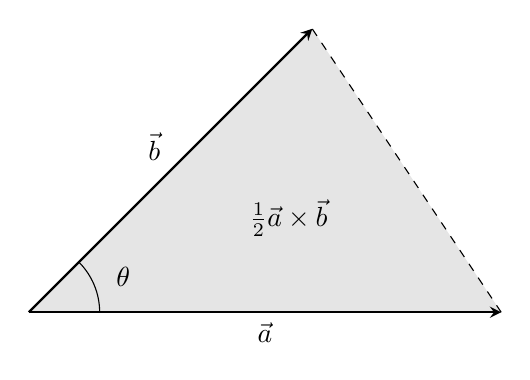
\begin{tikzpicture}[scale=3,>=stealth]
\coordinate (O) at (0,0);
\coordinate (A) at (2,0);
\coordinate (B) at (1.2,1.2);
\coordinate (H) at (1.2,0);

\fill[gray!20] (O) -- (A) -- (B) -- cycle;

\draw (0.3,0) arc (0:45:0.3);
\node at (0.4,0.15) {$\theta$};

\node at (1.1,0.4) {$\frac{1}{2}\abs{\vec{a} \times \vec{b}}$};
\draw[->, thick] (O) -- (A) node[midway, below] {$\vec{a}$};
\draw[->, thick] (O) -- (B) node[midway, above left] {$\vec{b}$};
\draw[dashed] (A) -- (B);
\end{tikzpicture}
\end{center}
We can also fix a vector $\vec{a}$ and consider $\vec{a} \perp \vec{x}$. Then computing $\vec{a} \times \vec{x}$ gives another vector that scales $\vec{x}$ by the $|\vec{a}|$ and rotates it by $\pi/2$ in a plane that is orthogonal to $\vec{a}$.

\subsection{Component Expressions}
For any right-handed orthonormal basis we have that:
\begin{align*}
  \vec{e}_1 \times \vec{e}_2 &= \vec{e}_3 = -\vec{e}_2 \times \vec{e}_1 \\
  \vec{e}_2 \times \vec{e}_3 &= \vec{e}_1 = -\vec{e}_3 \times \vec{e}_2 \\
  \vec{e}_3 \times \vec{e}_1 &= \vec{e}_2 = -\vec{e}_3 \times \vec{e}_1
\end{align*}
Consider $\vec{a} = (a_1, a_2, a_3)$ and $\vec{b} = (b_1, b_2, b_3)$ then:
\begin{align*}
  \vec{a} \times \vec{b} &= (a_1 \vec{e}_1 + a_2 \vec{e}_2 + a_3 \vec{e}_3) \times (b_1 \vec{e}_1 + b_2 \vec{e}_2 + b_3 \vec{e}_3) \\
                         &= (a_1 b_2 \vec{e}_3 - a_1 b_3 \vec{e}_2 - a_2 b_1 \vec{e}_3 + a_2 b_3 \vec{e}_1 + a_3 b_1 \vec{e}_2 - a_3 b_2 \vec{e}_1) \\
                         &= (a_2 b_3 - a_3 b_2) \vec{e}_1 + (a_3 b_1 - a_1 b_3) \vec{e}_2 + (a_1 b_2 - a_2 b_1) \vec{e}_3
\end{align*}
We can also write this as a matrix determinant:
\[
  \vec{a} \times \vec{b} =\begin{vmatrix}
  \vec{e}_1 & \vec{e}_2 & \vec{e}_3 \\
  a_1 & a_2 & a_3 \\
  b_1 & b_2 & b_3 \\
  \end{vmatrix}
\]
\section{Triple Products}
\begin{remark}[Note]
For this section, consider vectors in $\R^{3}$ only.
\end{remark}
\subsection{Scalar Triple Product}
\begin{definition}
  Consider $\vec{a}, \vec{b}, \vec{c}$ then the \textit{scalar triple product} is:
  \[
    [\vec{a}, \vec{b}, \vec{c}] = \vec{a} \cdot (\vec{b} \times \vec{c})
  \]
\end{definition}
Cyclic permutations of $\vec{a}, \vec{b}, \vec{c}$ retain the value of the scalar triple product and then swapping any two elements otherwise introduces a minus sign:
\begin{align*}
  &\vec{a} \cdot (\vec{b} \times \vec{c}) = \vec{b} \cdot (\vec{c} \times \vec{a}) = \vec{c} \cdot (\vec{a} \times \vec{b}) \\
  &= -\vec{a} \cdot (\vec{c} \times \vec{b}) = -\vec{b} \cdot (\vec{a} \times \vec{c}) = -\vec{c} \cdot (\vec{b} \times \vec{a})
\end{align*}
Geometrically, $|\vec{a} \cdot (\vec{b} \times \vec{c})|$ is the volume of the parallelepiped with sides $\vec{a}$, $\vec{b}$, $\vec{c}$.
\[
  |\vec{a} \cdot (\vec{b} \times \vec{c})| = (\text{area of base}) \times(\text{perpendicular height}) = \text{volume}
\]
If this is taken without the modulus then $\vec{a} \cdot (\vec{b} \times \vec{c})$ is a signed volume.
\begin{itemize}
  \item $\vec{a} \cdot (\vec{b} \times \vec{c}) > 0$ then $\vec{a}, \vec{b}, \vec{c}$ constitute a right handed set.
  \item $\vec{a} \cdot (\vec{b} \times \vec{c}) < 0$ then $\vec{a}, \vec{b}, \vec{c}$ constitute a left handed set.
  \item $\vec{a} \cdot (\vec{b} \times \vec{c}) = 0$ if and only if $\vec{a}, \vec{b}, \vec{c}$ are coplanar. That is, one of them is a linear combination of the other two.
\end{itemize}
\subsection{Vector Triple Product}
\begin{definition}[Vector Triple Product]
  $\vec{a}, \vec{b}, \vec{c} \in \R^{3}$ then the \textit{vector triple product} is:
  \[
    \vec{a} \times (\vec{b} \times \vec{c}) = (\vec{a} \cdot \vec{c}) \vec{b} - (\vec{a} \cdot \vec{b}) \vec{c}
  \]
\end{definition}
\begin{remark}[Warning]
  In general the vector triple product is not associative:
  \begin{align*}
    \vec{a} \times (\vec{b} \times \vec{c}) &= (\vec{a} \cdot \vec{c}) \vec{b} - (\vec{a} \cdot \vec{b})\vec{c} \\
    (\vec{a} \times \vec{b}) \times \vec{c} &= (\vec{a} \cdot \vec{c}) \vec{b} - (\vec{b} \cdot \vec{c})\vec{a}
  \end{align*}
\end{remark}
\section{Lines, Planes, and Vector Equations}
\subsection{Lines}
Any point on the line through a point $\vec{a}$ with direction $\vec{u}$ ($\vec{u} \neq 0$) has position vector given by:
\[
  \vec{r} = \vec{a} + \lambda \vec{u} \quad \lambda \in \R
\]

\begin{center}
\begin{tikzpicture}[scale=2,>=stealth]
  \coordinate (O) at (0.6,-0.5);
  \coordinate (A) at (0,0);
  \coordinate (B) at (2.4,1.2);
  \coordinate (C) at (1.2,0.6);

  \draw[dashed, gray] (-1.6,-0.8) -- (3,1.5);

  \draw[->, thick, black] (A) -- (C) node[midway, above left] {$\vec{u}$};
  \draw[->, thick, black] (O) -- (A) node[midway, above right] {$\vec{a}$};
  \draw[->, thick, black] (O) -- (B) node[midway, below right] {$\vec{r}$};
  \draw[->, black] (A) -- (B) node[near end, above left] {$\lambda \vec{u}$};


  \fill (O) circle (0.03);
  \node[below right] at (O) {$O$};
  \node[above left] at (A) {$A$};
\end{tikzpicture}
\end{center}
We can rearrange this to get:
\begin{align*}
  (\vec{r} - \vec{a}) &= \lambda \vec{u} \\
  (\vec{r} - \vec{a}) \times \vec{u} &= \vec{0}
\end{align*}
or equivalently $\vec{r} \times \vec{u} = \vec{b}$.
\subsection{Planes}
Any point on a plane though $\vec{a}$ with two direction vectors $\vec{u}$, $\vec{v}$ ($\vec{u} \centernot\parallel \vec{v}$) has position vector given by:
\[
  \vec{r} = \vec{a} + \lambda \vec{u} + \mu \vec{v} \quad \lambda, \mu \in \R
\]
A vector normal to the plane is given by $\vec{n} = \vec{u} \times \vec{v}$. Then we can write:
\[
  \vec{r} \cdot \vec{n} = \vec{a} \cdot \vec{n} \text{ or } (\vec{r} - \vec{a}) \cdot \vec{n} = 0
\]
The component of $\vec{r}$ along $\vec{n}$ is
\[
  \uvec{n} \cdot \vec{r} = \frac{\vec{n} \cdot \vec{r}}{|\vec{n}|} = \frac{k}{|\vec{n}|}
\]
which is also the perpendicular distance from the origin to the plane.

If $\vec{a}, \vec{b}, \vec{c}$ are coplanar, then we can write the plane containing them as:
\[
  (\vec{r} - \vec{a}) \cdot [(\vec{b} - \vec{a}) \times (\vec{c} - \vec{a})] = 0
\]
\begin{example}[Finding the Intersection Between a Line and a Plane]
  Consider a line given by $\vec{u} \times \vec{r} = \vec{u} \times \vec{a}$ and a plane given by $\vec{n} \cdot \vec{r} = \vec{n} \cdot \vec{b}$.

  The line can also be written as $\vec{r} \times \vec{u} = \vec{a} \times \vec{u}$.
  Taking the vector product of this with $\vec{n}$ yields:
  \begin{align*}
    (\vec{a} \times \vec{u}) \times \vec{n} &= (\vec{r} \times \vec{u}) \times \vec{n}\\
                                            &= (\vec{r} \cdot \vec{n}) \vec{u} - (\vec{u} \cdot \vec{n}) \vec{r} \text{ by vector triple product}\\
                                            &= (\vec{b} \cdot \vec{n}) \vec{u} - (\vec{u} \cdot \vec{n}) \vec{r} \text{ by definition of plane}\\
    (\vec{u} \cdot \vec{n})\vec{r} &= (\vec{b} \cdot \vec{n}) \vec{u} - (\vec{a} \times \vec{u}) \times \vec{n}\\
    \vec{r} &= \frac{(\vec{b} \cdot\vec{n})\vec{u} - (\vec{a} \times \vec{u})\times\vec{n}}{\vec{u} \cdot\vec{n}} \text{ provided $\vec{u} \cdot \vec{n} = 0$}
  \end{align*}
  In the case that $\vec{u} \cdot \vec{n} = 0$ then $\vec{u}$ is orthogonal to $\vec{n}$ so either:
  \begin{itemize}
    \item The line and plane are parallel so never intersect
    \item The line is contained entirely within the plane so the intersection is just the line itself.
  \end{itemize}
\end{example}
\end{document}
